\gls{tic} gives the possibility to analyse time course RNA-Seq data starting from \textit{BAM} files.
It enables RNA expression quantification with \lstinline!featureCounts! method producing a count matrix useful for \glspl{deg} detection.

We gave particular attention to the normalization phase, giving the possibliity not only to use several traditional normalizations methods, but also the possiblity to remove batch effect.


\begin{figure}[H]
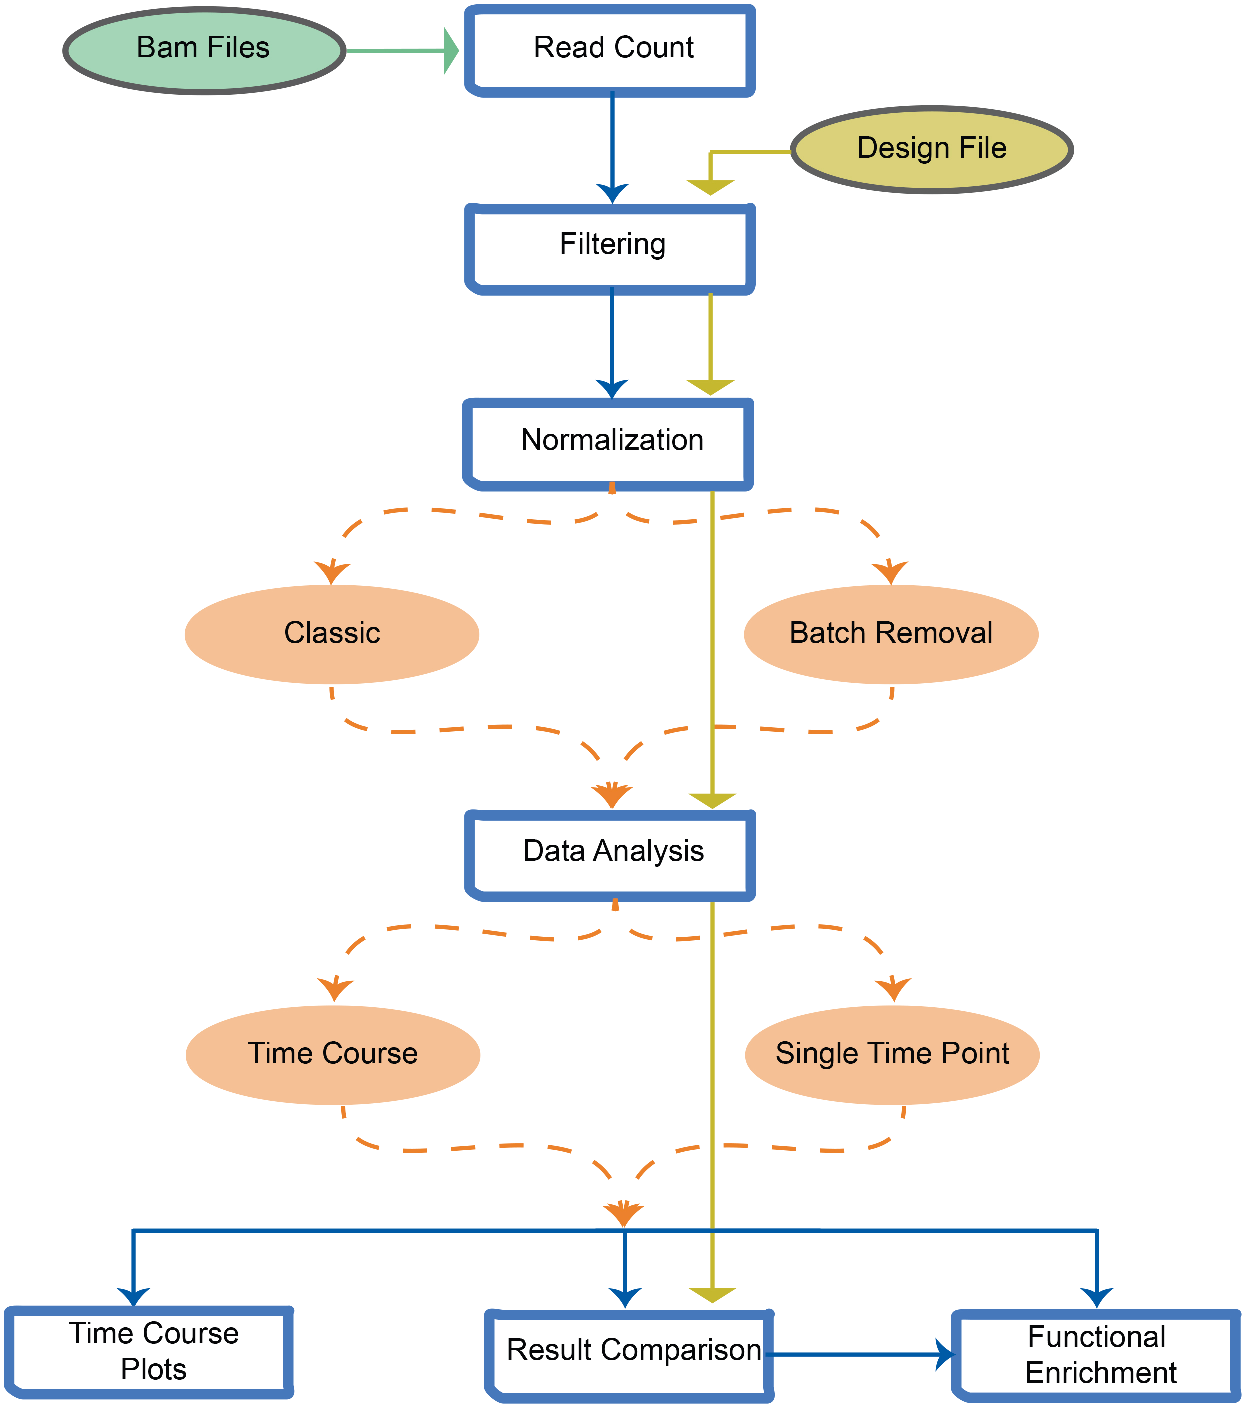
\includegraphics[width=\textwidth,height=\textheight,keepaspectratio]{img/ticorser/main_flow.pdf}
\caption[ticorser mainflow]{Main flow of ticorser R package.}
\label{fig:ticorserflow}
\centering
\end{figure}

\gls{tic} offers four different ways for analyzing time course RNA-Seq data.

Moreover, it offers three different ways for analyzing different biological conditions in a single time point.